\SourcePage{102}{105}
\section{Transmission Coefficient}

We consider particle motion in a field of the type depicted in Fig.~5:
$U(x)$ increases monotonically from one constant limiting value ($U=0$ as
$x\to-\infty$) to another ($U=U_0$ as $x\to+\infty$). According to
classical mechanics, a particle with energy $E<U_0$ moving in such a field
from left to right arrives at the \emph{potential wall}, reflects off it,
and proceeds in the reverse
\SourcePage{103}{106}
direction; for $E>U_0$, however, the particle keeps traveling in its original
direction with a reduced velocity. Quantum mechanics introduces a new
phenomenon: even when $E>U_0$, the particle may be reflected from the
potential wall. In principle, the reflection probability is to be calculated
as follows.

\begin{center}
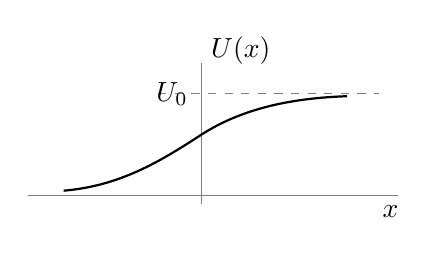
\begin{tikzpicture}[x=1.0cm,y=0.75cm]
  \draw[gray] (-2.2,0)--(2.5,0);
  \draw[gray] (0,-0.15)--(0,2.25);
  \draw[dashed,gray] (-0.55,1.72)--(2.25,1.72);
  \draw[thick] (-1.75,0.08)
    .. controls (-1.05,0.16) and (-0.55,0.55) .. (0,1.03)
    .. controls (0.55,1.50) and (1.20,1.65) .. (1.85,1.68);
  \node[above right] at (0,2.05) {$U(x)$};
  \node[left] at (-0.05,1.72) {$U_0$};
  \node[below] at (2.4,0) {$x$};
\end{tikzpicture}

\small Figure~5
\end{center}

Let the particle move from left to right. At large positive values of $x$,
the wave function must describe a particle that has passed ``over the wall''
and is moving in the positive direction of the $x$ axis; that is, it must
have the asymptotic form
\begin{equation}
  \text{as }x\to\infty:\qquad
  \psi\approx Ae^{ik_2x},
  \qquad k_2=\frac{1}{\hbar}\sqrt{2m(E-U_0)}
  \tag{25.1}
\end{equation}
($A$ is a constant). Having found a solution of the Schrödinger equation
that satisfies this limiting condition, we calculate its asymptotic
expression as $x\to-\infty$. This is a linear combination of two solutions
of the free-motion equation and therefore has the form
\begin{equation}
  \text{as }x\to-\infty:\qquad
  \psi\approx e^{ik_1x}+Be^{-ik_1x},
  \qquad k_1=\frac{1}{\hbar}\sqrt{2mE}.
  \tag{25.2}
\end{equation}
The first term describes the particle impinging on the wall ($\psi$ is taken
normalized so that this term has unit coefficient); the second term depicts
the particle reflected from the wall. The flux density is
proportional to $k_1$ in the incident wave, to $k_1|B|^2$ in the reflected
wave, and to $k_2|A|^2$ in the transmitted wave. Define the particle's
\emph{transmission coefficient} $D$ as the ratio of the flux density in the
transmitted wave to that in the incident wave:
\begin{equation}
  D=\frac{k_2}{k_1}|A|^2.
  \tag{25.3}
\end{equation}
Similarly, the \emph{reflection coefficient} $R$ may be defined as the ratio
of the reflected flux density to the incident flux density; evidently
$R=1-D$:
\begin{equation}
  R=|B|^2=1-\frac{k_2}{k_1}|A|^2
  \tag{25.4}
\end{equation}
(this relation between $A$ and $B$ follows automatically from the constancy
of the flux along the $x$ axis).

If a particle moves from left to right with energy $E<U_0$, then $k_2$ is
purely imaginary and the wave function decreases exponentially as
$x\to+\infty$. The reflected flux equals the incident flux; that is,
\SourcePage{104}{107}
the particle is totally reflected from the potential wall. We stress,
however, that the probability for the particle to be located in the region
$E<U$ remains nonzero even in this case, though it decreases
rapidly with growing $x$.

For the general case of an arbitrary stationary state (energy $E>U_0$),
the asymptotic form of the wave function both as $x\to-\infty$ and as
$x\to+\infty$ is a sum of two waves propagating in the two directions along
the $x$ axis:
\begin{equation}
  \begin{aligned}
    \psi&=A_1e^{ik_1x}+B_1e^{-ik_1x} &&\text{as }x\to-\infty,\\
    \psi&=A_2e^{ik_2x}+B_2e^{-ik_2x} &&\text{as }x\to+\infty.
  \end{aligned}
  \tag{25.5}
\end{equation}
Since both expressions are asymptotic forms of one and the same solution of
a linear differential equation, the coefficients $A_1$, $B_1$ and $A_2$,
$B_2$ are linearly related. Let
$A_2=\alpha A_1+\beta B_1$, where $\alpha$ and $\beta$ are constants (in
general complex) that depend on the particular form of the field $U(x)$.
The analogous relation for $B_2$ may then be written by using the fact that
the Schrödinger equation is real. By this fact, if $\psi$ is a solution of
the given Schrödinger equation, the complex-conjugate function $\psi^*$ is
also a solution of the same equation.

The asymptotic form
\[
  \begin{aligned}
    \psi^*&=A_1^*e^{-ik_1x}+B_1^*e^{ik_1x} &&\text{as }x\to-\infty,\\
    \psi^*&=A_2^*e^{-ik_2x}+B_2^*e^{ik_2x} &&\text{as }x\to+\infty
  \end{aligned}
\]
differs from (25.5) only in the notation of the constant coefficients;
hence $B_2^*=\alpha B_1^*+\beta A_1^*$, or
$B_2=\alpha^*B_1+\beta^*A_1$. Thus the coefficients in (25.5) are related
by equations of the form
\begin{equation}
  A_2=\alpha A_1+\beta B_1,
  \qquad B_2=\beta^*A_1+\alpha^*B_1.
  \tag{25.6}
\end{equation}

The condition that the flux be constant along the $x$ axis gives the
following relation for the coefficients in (25.5):
\[
  k_1\bigl(|A_1|^2-|B_1|^2\bigr)
  =k_2\bigl(|A_2|^2-|B_2|^2\bigr).
\]
On expressing $A_2$ and $B_2$ here in terms of $A_1$ and $B_1$ according to
(25.6), we obtain
\begin{equation}
  |\alpha|^2-|\beta|^2=\frac{k_1}{k_2}.
  \tag{25.7}
\end{equation}

The relations (25.6) can be used to show that the reflection coefficients
are identical (at a given energy $E>U_0$) for particles propagating in the positive
or negative
\SourcePage{105}{108}
direction along the $x$ axis. Indeed, the first case is obtained by setting
$B_2=0$ in the functions (25.5); then
$B_1/A_1=-\beta^*/\alpha^*$. In the second case we put $A_1=0$, whereupon
$A_2/B_2=\beta/\alpha^*$. The corresponding reflection coefficients are
\[
  R_1=\left|\frac{B_1}{A_1}\right|^2
  =\left|\frac{\beta^*}{\alpha^*}\right|^2,
  \qquad
  R_2=\left|\frac{A_2}{B_2}\right|^2
  =\left|\frac{\beta}{\alpha^*}\right|^2,
\]
and it is clear that $R_1=R_2$.

The quantities $B_1/A_1=-\beta^*/\alpha^*$ and
$A_2/B_2=\beta/\alpha^*$ are naturally called the \emph{reflection
amplitudes} for motion in the positive and negative directions,
respectively. These amplitudes have equal moduli but may differ by a phase
factor.

\ProblemHeading
\textbf{1.} For a particle with energy $E>U_0$, calculate the coefficient of
reflection from a rectangular potential wall (Fig.~6).

\begin{center}
\begin{tikzpicture}[x=1.0cm,y=0.7cm]
  \draw[gray] (-1.8,0)--(2.2,0);
  \draw[gray] (0,-0.2)--(0,2.2);
  \draw[thick] (-1.45,0)--(0,0)--(0,1.35)--(1.55,1.35);
  \node[above right] at (0,2.0) {$U(x)$};
  \node[left] at (0,1.35) {$U_0$};
  \node[below] at (2.1,0) {$x$};
\end{tikzpicture}

\small Figure~6
\end{center}

\SolutionHeading
Throughout the region $x>0$ the wave function has the form (25.1), and in
the region $x<0$ it has the form (25.2). The constants $A$ and $B$ are
determined by the conditions that $\psi$ and $d\psi/dx$ be continuous at
$x=0$:
\[
  1+B=A,\qquad k_1(1-B)=k_2A,
\]
whence
\[
  A=\frac{2k_1}{k_1+k_2},
  \qquad B=\frac{k_1-k_2}{k_1+k_2}.
\]
The reflection coefficient is (25.4)
\footnote{In the limiting case of classical mechanics the reflection
coefficient must go to zero. However, the resulting expression does not
contain a quantum constant at all. This seeming contradiction is resolved
as follows. The classical limit corresponds to the situation where the particle's de Broglie wavelength
$\lambda\sim\hbar/p$ is small in comparison with the characteristic
dimensions of the problem, that is, with the distances over which the field
$U(x)$ changes appreciably. In the schematic example under consideration
this distance is zero (at $x=0$), so that the limiting transition cannot be
made.}
\[
  R=\left(\frac{k_1-k_2}{k_1+k_2}\right)^2
  =\left(\frac{p_1-p_2}{p_1+p_2}\right)^2.
\]
At $E=U_0$ ($k_2=0$), $R$ becomes unity; as $E\to\infty$, it tends to zero
as $R=(U_0/4E)^2$.

\ProblemHeading
\textbf{2.} Determine the transmission coefficient of a particle through a
rectangular potential barrier (Fig.~7).

\SolutionHeading
Let $E>U_0$, and let the incident particle move from left to right. The wave
function then has the following forms in the different regions:
\[
  \begin{aligned}
    \psi&=e^{ik_1x}+Ae^{-ik_1x} &&\text{for }x<0,\\
    \psi&=Be^{ik_2x}+B'e^{-ik_2x} &&\text{for }0<x<a,\\
    \psi&=Ce^{ik_1x} &&\text{for }x>a.
  \end{aligned}
\]
\SourcePage{106}{109}
(On the side $x>a$ there must be only the transmitted wave, propagating in
the positive direction of the $x$ axis.) The constants $A$, $B$, $B'$, and
$C$ are determined by the conditions that $\psi$ and $d\psi/dx$ be
continuous at the points $x=0,a$. The transmission coefficient is
$D=k_1|C|^2/k_1=|C|^2$. Calculation gives
\[
  D=\frac{4k_1^2k_2^2}
  {(k_1^2-k_2^2)^2\sin^2ak_2+4k_1^2k_2^2}.
\]

\begin{center}
\begin{tikzpicture}[x=1.0cm,y=0.72cm]
  \draw[gray] (-1.7,0)--(2.5,0);
  \draw[gray] (0,-0.2)--(0,2.2);
  \draw[thick] (-1.45,0)--(0,0)--(0,1.35)--(1.45,1.35)--(1.45,0)--(2.2,0);
  \node[above right] at (0,2.0) {$U(x)$};
  \node[left] at (0,1.35) {$U_0$};
  \node[below] at (1.45,0) {$a$};
\end{tikzpicture}

\small Figure~7
\end{center}

When $E<U_0$, $k_2$ is purely imaginary; the corresponding expression for
$D$ is obtained by replacing $k_2$ by $i\kappa_2$, where
$\hbar\kappa_2=\sqrt{2m(U_0-E)}$:
\[
  D=\frac{4k_1^2\kappa_2^2}
  {(k_1^2+\kappa_2^2)^2\sinh^2(a\kappa_2)
    +4k_1^2\kappa_2^2}.
\]

\ProblemHeading
\textbf{3.} Determine the reflection coefficient of a particle from the
potential wall defined by
\[
  U(x)=U_0/(1+e^{-\alpha x})
\]
(see Fig.~5); the particle energy is $E>U_0$.

\SolutionHeading
The Schrödinger equation is
\[
  \frac{d^2\psi}{dx^2}+\frac{2m}{\hbar^2}
  \left(E-\frac{U_0}{1+e^{-\alpha x}}\right)\psi=0.
\]
We must find the solution that, as $x\to+\infty$, has the form
\[
  \psi=\operatorname{const}\cdot e^{ik_2x}.
\]
Introduce the new variable
\[
  \xi=-e^{-\alpha x}
\]
(which ranges from $-\infty$ to 0), and seek a solution in the form
\[
  \psi=\xi^{-ik_2/\alpha}w(\xi),
\]
where $w(\xi)$ tends to a constant as $\xi\to0$ (that is, as
$x\to\infty$). For $w(\xi)$ we obtain an equation of hypergeometric type,
\[
  \xi(1-\xi)w''+
  \left(1-\frac{2i}{\alpha}k_2\right)(1-\xi)w'
  +\frac{1}{\alpha^2}(k_2^2-k_1^2)w=0,
\]
whose solution is the hypergeometric function
\[
  w=F\left[-\frac{i}{\alpha}(k_1-k_2),
  -\frac{i}{\alpha}(k_1+k_2),-\frac{2i}{\alpha}k_2+1,\xi\right]
\]
(a constant factor is omitted). As $\xi\to0$, this function tends to 1 and
thus satisfies the stated condition.

The asymptotic form of $\psi$ as $\xi\to-\infty$ (that is, as
$x\to-\infty$) is
\footnote{See formula (e.6), in each of whose two terms only the first term
of the expansion is to be retained; that is, the hypergeometric functions
of $1/z$ are to be replaced by unity.}
\[
  \begin{aligned}
  \psi&\approx\xi^{-ik_2/\alpha}
  \left[C_1(-\xi)^{i(k_2-k_1)/\alpha}
       +C_2(-\xi)^{i(k_1+k_2)/\alpha}\right]\\
  &=(-1)^{ik_2/\alpha}\left[C_1e^{ik_1x}+C_2e^{-ik_1x}\right],
  \end{aligned}
\]
\SourcePage{107}{110}
where
\[
  C_1=\frac{\Gamma(-(2i/\alpha)k_1)\Gamma(-(2i/\alpha)k_2+1)}
  {\Gamma(-(i/\alpha)(k_1+k_2))
   \Gamma(-(i/\alpha)(k_1+k_2)+1)},
\]
\[
  C_2=\frac{\Gamma((2i/\alpha)k_1)\Gamma(-(2i/\alpha)k_2+1)}
  {\Gamma((i/\alpha)(k_1-k_2))
   \Gamma((i/\alpha)(k_1-k_2)+1)}.
\]
The required reflection coefficient is $R=|C_2/C_1|^2$; calculation using
the familiar formula
\[
  \Gamma(x)\Gamma(1-x)=\frac{\pi}{\sin\pi x}
\]
gives
\[
  R=\left\{
  \frac{\sinh[(\pi/\alpha)(k_1-k_2)]}
       {\sinh[(\pi/\alpha)(k_1+k_2)]}
  \right\}^2.
\]
At $E=U_0$ ($k_2=0$), $R$ becomes unity, while as $E\to\infty$ it tends
to zero according to
\[
  R=\left(\frac{\pi U_0}{\alpha\hbar}\right)^2
  \frac{2m}{E}\exp\left(-\frac{4\pi}{\alpha\hbar}\sqrt{2mE}\right).
\]
In the limiting transition to classical mechanics, $R$ vanishes, as it
should.

\ProblemHeading
\textbf{4.} Determine the transmission coefficient of a particle through
the potential barrier defined by
\[
  U(x)=\frac{U_0}{\cosh^2(\alpha x)}
\]
(Fig.~8); the particle energy is $E<U_0$.

\begin{center}
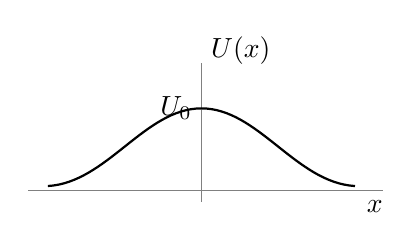
\begin{tikzpicture}[x=1.0cm,y=0.72cm]
  \draw[gray] (-2.2,0)--(2.3,0);
  \draw[gray] (0,-0.2)--(0,2.25);
  \draw[thick] (-1.95,0.08)
    .. controls (-1.20,0.14) and (-0.72,1.45) .. (0,1.45)
    .. controls (0.72,1.45) and (1.20,0.14) .. (1.95,0.08);
  \node[above right] at (0,2.05) {$U(x)$};
  \node[left] at (0,1.45) {$U_0$};
  \node[below] at (2.2,0) {$x$};
\end{tikzpicture}

\small Figure~8
\end{center}

\SolutionHeading
The Schrödinger equation for this problem is obtained from the example
considered in Problem 5 of \secref{23} by changing the sign of $U_0$, with the
energy $E$ now taken to be positive.

The same method gives the solution
\begin{equation}
  \psi=(1-\xi^2)^{-ik/2\alpha}
  F\left(-\frac{ik}{\alpha}-s,-\frac{ik}{\alpha}+s+1,
  -\frac{ik}{\alpha}+1,\frac{1-\xi}{2}\right),
  \tag{1}
\end{equation}
where
\[
  \xi=\tanh(\alpha x),\qquad
  k=\frac{1}{\hbar}\sqrt{2mE},\qquad
  s=\frac12\left(-1+\sqrt{1-\frac{8mU_0}{\alpha^2\hbar^2}}\right).
\]
This solution already satisfies the condition that as $x\to\infty$ (that
is, as $\xi\to1$, $(1-\xi)\approx2e^{-2\alpha x}$) the wave function
contain only the transmitted wave ($\sim e^{ikx}$). The asymptotic expression for
the wave function as $x\to-\infty$ ($\xi\to-1$) is obtained by transforming
the hypergeometric function via formula (e.7):
\begin{equation}
  \psi\sim e^{-ikx}\frac{\Gamma(ik/\alpha)\Gamma(1-ik/\alpha)}
  {\Gamma(-s)\Gamma(1+s)}
  +e^{ikx}\frac{\Gamma(-ik/\alpha)\Gamma(1-ik/\alpha)}
  {\Gamma(-ik/\alpha-s)\Gamma(-ik/\alpha+s+1)}.
  \tag{2}
\end{equation}
\SourcePage{108}{111}
Taking the squared modulus of the ratio of the coefficients in this
function, we obtain the following expression for the transmission
coefficient $D=1-R$:
\[
  D=\frac{\sinh^2(\pi k/\alpha)}
  {\sinh^2(\pi k/\alpha)+
   \cos^2\left(\frac{\pi}{2}
   \sqrt{1-\frac{8mU_0}{\hbar^2\alpha^2}}\right)}
  \quad\text{when}\quad \frac{8mU_0}{\hbar^2\alpha^2}<1,
\]
\[
  D=\frac{\sinh^2(\pi k/\alpha)}
  {\sinh^2(\pi k/\alpha)+
   \cosh^2\left(\frac{\pi}{2}
   \sqrt{\frac{8mU_0}{\hbar^2\alpha^2}-1}\right)}
  \quad\text{when}\quad \frac{8mU_0}{\hbar^2\alpha^2}>1.
\]
The first of these formulas also applies when $U_0<0$, that is, when the
particle passes not over a potential barrier but over a potential well. It
is noteworthy that then $D=1$ if
$1+(8m|U_0|/\hbar^2\alpha^2)=(2n+1)^2$; thus, for certain values of the well
depth $|U_0|$, particles passing over it are not reflected. This is already
clear from expression (2), in which the term containing $e^{-ikx}$ is
entirely absent when $s$ is a positive integer.

\ProblemHeading
\textbf{5.} Determine how the transmission coefficient tends to zero as
$E\to0$, assuming that the potential energy $U(x)$ decreases rapidly at
distances $|x|\gg a$, where $a$ is the characteristic size of the
interaction region.

\SolutionHeading
In the range of distances $k|x|\ll1$, the energy $E$ may be neglected in
the Schrödinger equation. If also $|x|\gg a$, the potential energy may be
neglected as well, and the equation reduces to
\[
  -\frac{\hbar^2}{2m}\frac{d^2\psi}{dx^2}=0,
\]
whose solution we write as
\begin{equation}
  \psi=a_1+b_1x,\quad x<0,
  \qquad \psi=a_2+b_2x,\quad x>0.
  \tag{1}
\end{equation}
Solving the equation at distances $|x|\sim a$ determines the relation among
$a_1$, $b_1$ and $a_2$, $b_2$. This relation is linear and has the form
\begin{equation}
  a_1=\rho a_2+\mu b_2,
  \qquad b_1=\nu a_2+\tau b_2.
  \tag{2}
\end{equation}
The coefficients $\rho$, $\mu$, $\nu$, and $\tau$ are real and independent
of the energy, since the energy no longer enters the equation
\footnote{By constancy of the flux, they satisfy
$\rho\tau-\mu\nu=1$.}.
Solution (1) must agree with the first two terms in the expansions of
(25.1) and (25.2) in powers of $x$, whence
\[
  a_1=1+B,\qquad b_1=ik(1-B),\qquad a_2=A,\qquad b_2=ikA.
\]
Substituting these expressions in (2) and solving the equations for $A$, we
find, at small $k$, $A\approx2ik/\nu$, whence
\[
  D\approx\frac{4k^2}{\nu^2}\sim E.
\]
Thus the transmission coefficient tends to zero in proportion to the
particle energy. This general relation is, of course, satisfied in the
examples considered in Problems 2 and 4.
